%%%%%%%%%%%%%%%%%%%%%%%%%%%%%%%%%%%%%%%%%
% Simple Sectioned Essay Template
% LaTeX Template
%
% This template has been downloaded from:
% http://www.latextemplates.com
%
% Note:
% The \lipsum[#] commands throughout this template generate dummy text
% to fill the template out. These commands should all be removed when 
% writing essay content.
%
%%%%%%%%%%%%%%%%%%%%%%%%%%%%%%%%%%%%%%%%%

%----------------------------------------------------------------------------------------
%	PACKAGES AND OTHER DOCUMENT CONFIGURATIONS
%----------------------------------------------------------------------------------------

\documentclass[11pt]{article} % Default font size is 12pt

\usepackage[utf8]{inputenc}

\usepackage[a4paper]{geometry} % Required to change the page size to A4
% Set the page size to be A4 as opposed to the default US Letter

\usepackage{subcaption} 
\usepackage{float} % Allows putting an [H] in \begin{figure} to specify the exact location of the figure
\usepackage{wrapfig} % Allows in-line images such as the example fish picture

\usepackage{lipsum} % Used for inserting dummy 'Lorem ipsum' text into the template

\usepackage{amsmath}

\usepackage{amsthm}
\theoremstyle{plain}
\newtheorem{theorem}{Theorem}[section]
\newtheorem{corollary}{Corollary}[theorem]
\newtheorem{proposition}[theorem]{Proposition}
\newtheorem{lemma}[theorem]{Lemma}

\theoremstyle{definition}
\newtheorem{definition}{Definition}[section]

\theoremstyle{remark}
\newtheorem*{remark}{Remark}

\usepackage{amssymb}

\usepackage{dsfont}

\usepackage{epigraph}

\usepackage[numbers, sort]{natbib}
\bibliographystyle{plainnat}

\usepackage[nottoc]{tocbibind}

\usepackage{makeidx}
\makeindex

\linespread{1.2} % Line spacing

\setlength\parindent{0pt} % Uncomment to remove all indentation from paragraphs
\setlength{\parskip}{8pt}

\usepackage{graphicx} % Required for including pictures
\graphicspath{{../figures/}} % Specifies the directory where pictures are stored

\usepackage{epstopdf}

\usepackage{hyperref}
\hypersetup{
    colorlinks,
    citecolor=black,
    filecolor=black,
    linkcolor=black,
    urlcolor=black
}

\usepackage{microtype}
\usepackage{siunitx}
\usepackage{cleveref}
\usepackage{booktabs}

\usepackage{todonotes}

\begin{document}

%----------------------------------------------------------------------------------------
%	TITLE PAGE
%----------------------------------------------------------------------------------------

\begin{titlepage}

\newcommand{\HRule}{\rule{\linewidth}{0.5mm}} % Defines a new command for the horizontal lines, change thickness here

\center % Center everything on the page

\textsc{\Large The University of New South Wales}\\[0.2cm]
\textsc{\large School of Computer Science and Engineering}\\[1.5cm] % Name of your university/college

\textsc{\large Thesis Report - Part A}\\[0.5cm] % Major heading such as course name
\textsc{BSc Computer Science (Honours)}\\[0.5cm] % Minor heading such as course title

\HRule \\[0.4cm]
{ \LARGE \bfseries The Chromatic Derivatives and its Applications }\\[0.4cm] % Title of your document
\HRule \\[1.5cm]

\begin{minipage}[t]{0.4\textwidth}
\begin{flushleft} \large
\emph{Author:}\\
Louis \textsc{Tiao} % Your name
\end{flushleft}
\end{minipage}
~
\begin{minipage}[t]{0.5\textwidth}
\begin{flushright} \large
\emph{Supervisor:} \\
Dr. Aleksandar \textsc{Ignjatovi\'{c}} % Supervisor's Name
\\[0.5cm]
\emph{Assessor:} \\
Dr. Alan \textsc{Blair} % Assessor's Name
\end{flushright}
\end{minipage}\\[4cm]

{\large \today}\\[3cm] % Date, change the \today to a set date if you want to be precise

%\includegraphics{Logo}\\[1cm] % Include a department/university logo - this will require the graphicx package

\vfill % Fill the rest of the page with whitespace

\end{titlepage}

%----------------------------------------------------------------------------------------
%	TABLE OF CONTENTS
%----------------------------------------------------------------------------------------

\tableofcontents % Include a table of contents

\newpage % Begins the essay on a new page instead of on the same page as the table of contents 

%----------------------------------------------------------------------------------------
%	INTRODUCTION
%----------------------------------------------------------------------------------------

\section{Introduction} % Major section

It is no overstatement that the Nyquist-Shannon sampling theorem
 is indispensable to the fields of communication and signal processing. It 
allows us to convert continuous real-world analog signals into discrete signals, 
represented as a sequence a numbers, to then be processed and manipulated digitally on a 
computer - it makes digital signal processing possible, both in theory and in practice.

Let $f$ is a signal of finite energy bandlimited by $B$, i.e. $f$ is a continuous $L^2$ 
function whose Fourier transform has support within $[-B,B]$. We denote the class of
such functions $\mathbf{BL}(B)$. The interpolation (reconstruction) formula complementary to the 
sampling theorem, commonly known as the Whittaker–Shannon interpolation formula, is
given by
\begin{equation} \label{eq:whittaker_shannon}
  f(t) = \sum_{n=-\infty}^{\infty} f(n) \mathrm{sinc}(t-n)
\end{equation}
where $\mathrm{sinc}$ is the (normalized) cardinal sine function, defined by 
$\mathrm{sinc}(x)=\frac{\sin{\pi x}}{\pi x}$ for $x \neq 0$ and $\mathrm{sinc}(0)=1$.

This series expansion in \cref{eq:whittaker_shannon} can be seen as a case of a 
generalized Fourier series, with the complete orthonormal system of univariate functions 
$\{ \mathrm{sinc}(t-n) \}_{n\in\mathbb{Z}}$ as its basis. Roughly speaking, the interpolation
formula given by \cref{eq:whittaker_shannon} and Fourier series in general are said to
``global'' in the sense that it requires the samples of the signal at integer points of 
\todo{Formalize this a bit more eh} arbitrarily large absolute value, i.e. values at 
points spanning a large part of its domain. Additionally, the truncation error of Fourier 
series is \todo{there must be a better word} distributed along the domain of the function.

On the other hand, consider a signal $f \in \mathbf{BL}(\pi)$ which is an analytic function.
Its Taylor series expansion about point $t=t_0$ is given by
\begin{equation} \label{eq:taylor}
  f(t) = \sum_{n=0}^{\infty} f^{(n)}(t_0) \frac{(t-t_0)^n}{n!}
\end{equation}
We mainly consider the expansion about point $t_0=0$, which is also known as the Maclaurin series.
The Taylor series are said to ``local'' in the sense that values of the $n$th order derivatives 
$f^{(n)}(t_0)$ can be obtains by samples of the signal on an arbitrarily small neighborhood
of $t_0$. It is no surprise then that the truncation error of Taylor series is very small in the 
neighborhood on which it has been computed and grows dramatically as we move away from this neighborhood.

In stark contrast to the Shannon-Whittaker interpolation, the Taylors series, though 
instrumental in mathematical analysis, finds relatively limited use to digital signal 
processing, due to its multitude of shortcomings. We give a brief overview of these problems
now, and extend our discussion in section \todo{blah}.

\begin{enumerate}
  \item numerical evaluation of derivatives, let alone those of higher orders are
    highly sensitive to noise.
  \item the Taylor series expansion of a signal $f \in \mathbf{BL}(\pi)$ does not
    converge uniformly on $\mathbb{R}$.
  \item as mentioned already, truncation error of Taylor series accumulates quite rapidly.
  \item the Shannon-Whittaker interpolation of signal $f \in \mathbf{BL}(\pi)$ converges
    to $f$ in $\mathbf{BL}(\pi)$ while the truncations (approximation by finite sum) of the
    Taylor series expansion do not belong to $\mathbf{BL}(\pi)$.
  \item For any input signal $f \in \mathbf{BL}(\pi)$ to a continuous, linear, time-invariant 
    system $L$, its output can be characterized entirely by samples of the signal 
    and the impulse response of the system $L[\mathrm{sinc}]$. More concisely,
    \begin{equation}
      L[f](t) = \sum_{n=-\infty}^{\infty} f(n) L[\mathrm{sinc}](t-n)
    \end{equation}
    Nothing resembling this can be said of Taylor series expansions.
\end{enumerate}

In light of these problems, it is no wonder we see little application of Taylor series
in digital signal processing. This is a pity, because there are a number of (albeit unusual) 
problems in signal processing that require processing and analyzing signals on an extremely
local and almost microscopic level, such as designing signal processors that exploit 
the predictive properties of the signal, methods for image reconstruction problems that 
specifically depend on information from local regions of the images rather than from the 
image as a whole, and some adaptive filtering applications.

Since Taylor series cannot readily be applied, we must reconcile the local properties 
of the Taylor series with the ideal properties of the Fourier series that make it so 
crucial to digital signal processing.

To alleviate some of the problems that render Taylor series ineffective for signal processing, 
the \emph{chromatic derivatives} were introduced by Dr.~Ignjatovi\'{c} in 2000. Naturally, the
theory emerged in the conception of a novel switching amplifier which had the ability anticipate
(predict) future signal values by exploiting the local signal behavior.

The \emph{chromatic expansions}, complementary to the chromatic derivatives, were later introduced   
and several applications and novel techniques that harness the theory of chromatic derivatives
have been also been proposed. Some of these include the design of communication channel
equalizers, digital transceivers, image compression methods, etc.

The theory has since been generalized and extended to systems corresponding to several classical 
families of orthogonal polynomials and was cast in to the convention signal processing framework. 
More recently, the chromatic derivatives and expansions were generalized to 
higher dimensions. 

We believe (multidimensional) chromatic derivatives and expansions lends itself naturally
to many applications in important fields such as image processing. The exploration, 
conception and implementation of some these applications will be the subject of this thesis. 

This report is structured as follows. In section , we formally define the chromatic derivatives, 
specifically those associated with the Legendre polynomials. For a concise and more generalized
exposition of chromatic derivatives, please consult , which also forms the basis for portions 
of this present report. Continuing in section , discuss some of its properties, and contrast 
chromatic expansions with Taylor/Fourier series expansions with some examples. In section , 
we outline some of the image processing problems we intend to tackle and give a brief literature 
review of the conventional methods used to solve these problems. Lastly, in section  we propose 
our approach to solving these problems with the machinery of multidimensional chromatic derivatives, 
and roughly outline the plan to undertake our approach.

\newpage

\section{Background}

\subsection{Preliminaries}

The \emph{Legendre functions} are solutions to the \emph{Legendre differential 
equation}, which is the second-order ordinary differential equation

\begin{equation} \label{eq:legendre_de}
\frac{d}{dx}\left[(1-x^2)\frac{d}{dx}L_n(x)\right]+n(n+1)L_n(x)=0
\end{equation}

The \emph{Legendre polynomials}, also known as \emph{Legendre functions of the 
first kind}, satisfy the following recurrence relation:
\begin{align}
L_0(x)     &= 1 \\
L_1(x)     &= x \\
L_{n+1}(x) &= \frac{2n+1}{n+1} x L_n(x) - \frac{n}{n+1} L_{n-1}(x)
\end{align}
The Legendre polynomials are orthogonal (and complete) over the closed interval 
$[-1, 1]$
\begin{equation*}
  \frac{1}{2}\int_{-1}^{1} L_n(x)L_m(x) dx = \frac{1}{2n+1} \delta_{mn}
\end{equation*}
where $\delta_{ij}$ is the Kronecker delta:
\begin{equation}
  \delta_{ij} =
    \begin{cases}
     0       & \text{for } i \neq j, \\
     1       & \text{for } i = j.
    \end{cases}
\end{equation}
We can easily normalize and scale to obtain Legendre polynomials that are
orthogonal (and complete) over the closed interval $[-\pi,\pi]$
\begin{equation}
  P_n^L(x) = \sqrt{2n+1}L_n\left(\frac{x}{\pi}\right)
\end{equation}
so that 
\begin{equation*}
\frac{1}{2\pi} \int_{-\pi}^{\pi} P_n^L(x)P_m^L(x) dx = \delta_{mn}
\end{equation*}
Likewise, it satisfies the recurrence relation
\begin{align}
P_0^L(x)     &= 1 \\
P_1^L(x)     &= \frac{\sqrt{3}}{\pi} x \\
P_{n+1}^L(x) &= \frac{\sqrt{4(n+1)^2-1}}{(n+1) \pi} x P_n^L(x) - \frac{n\sqrt{4(n+1)^2-1}}{(n+1)\sqrt{4n^2-1}} P_{n-1}^L(x)
\end{align}
More concisely, we can define this as
\begin{align}
  P_{n+1}^L(x) = \frac{1}{\gamma_n} x P_n(x) - \frac{\gamma_{n-1}}{\gamma_n} P_{n-1}(x)
\end{align}
with $P_{-1}(x)=0, P_0(x)=1$, and
\begin{equation}
  \gamma_n = \frac{(n+1) \pi}{\sqrt{4(n+1)^2-1}}
\end{equation}
with $\gamma_{-1} = 1$.

\subsection{Chromatic derivatives}

\subsubsection{Definition}

The chromatic derivatives associated with Legendre polynomials are defined as
\begin{equation}
  \mathcal{K}_t^n = (-i)^n P_n^L \left (i \frac{d}{dt} \right )
\end{equation} 
When applied to univariate functions, there should be no ambiguity as to
which variable we are differentiating with respect to, so we can use Heaviside's
notation to denote the differential operator, i.e. $\mathcal{D} = \mathcal{D}_t 
= \frac{d}{dt}$. 

So now we have
\begin{equation}
  \mathcal{K}^n = (-i)^n P_n^L \left (i \mathcal{D} \right )
\end{equation}
and this of course satisfies the recurrence relation
\begin{equation}
  \mathcal{K}^{n+1} = \frac{1}{\gamma_n} \left ( \mathcal{D} \circ \mathcal{K}^n \right ) 
                        + \frac{\gamma_{n-1}}{\gamma_n} \mathcal{K}^{n-1}
\end{equation}
with $\mathcal{K}^{-1} = 0, \mathcal{K}^0 = \mathds{1}$ where $\mathds{1}$ is 
the identity operator and $\gamma_n$ are as defined as before. Note that 
$\mathcal{K}^{-1}$ signifies the constant 0 operator.

Now, it is easy to see that
\begin{equation}
  \mathcal{K}_t^n[e^{i\omega t}] = i^n P_n^L(\omega) e^{i\omega t}
\end{equation}
since the polynomials $P_n^L(x)$ contains only variables with powers of the same
parity as that of $n$, and the operators $\mathcal{K}_t^n$ have real coefficients.

Let $x(t) \in \mathbf{BL}(\pi)$. We now have,
\begin{align*}
  \mathcal{K}_t^n[x(t)]
    &= \mathcal{K}_t^n[\mathcal{F}^{-1}[X(\omega)]] \\
    &= \mathcal{K}_t^n \left [ \frac{1}{2 \pi} \int_{-\infty}^{\infty} X(\omega) e^{i \omega t} d\omega \right ] \\
    &= \frac{1}{2 \pi} \int_{-\infty}^{\infty} X(\omega) \mathcal{K}_t^n[e^{i \omega t}] d\omega \\
    &= \frac{1}{2 \pi} \int_{-\infty}^{\infty} i^n P_n^L(\omega) X(\omega) e^{i\omega t} d\omega \\
    &= \frac{1}{2 \pi} \int_{-\pi}^{\pi} i^n P_n^L(\omega) X(\omega) e^{i\omega t} d\omega \\
\end{align*}

\begin{remark}
We denote the Fourier transform and its inverse respectively as 
\begin{align}
  X(\omega) &= \mathcal{F}[x(t)] = \int_{-\infty}^{\infty} x(t) e^{-i \omega t} dt \\
  x(t)      &= \mathcal{F}^{-1}[X(\omega)] = \frac{1}{2 \pi} \int_{-\infty}^{\infty} X(\omega) e^{i \omega t} d\omega
\end{align}
\end{remark}

\subsubsection{Frequency response}

Systems (operators) can have a variety of effects on input signals of different frequencies, 
e.g. they may amplify certain frequency components while attenuating others. The \emph{frequency 
response} of a system is the way the system output relates to the system input signals for 
different frequencies in the frequency domain. More precisely, consider the input signal $X(\omega)$
in the frequency domain. Denote the system output as $Y(\omega)$. The frequency response $H(\omega)$ 
satisfies the relationship
\begin{equation}
  Y(\omega) = H(\omega) X(\omega)
\end{equation}
and is therefore given by
\begin{equation}
  H(\omega) = \frac{Y(\omega)}{X(\omega)}
\end{equation}
Let us now contrast the frequency response of the normalized $n$th order differential 
operator $\frac{1}{\pi^n} \frac{d^n}{dt^n} = \frac{1}{\pi^n} \mathcal{D}_t^n$ with that 
of the chromatic derivative operator $\mathcal{K}_t^n$.

Let $x(t) \in \mathbf{BL}(\pi)$,
\begin{align*}
  y(t) &= \frac{1}{\pi^n} \mathcal{D}_t^n[x(t)] \\
       &= \frac{1}{\pi^n} \mathcal{D}_t^n[\mathcal{F}^{-1}[X(\omega)]] \\
       &= \frac{1}{\pi^n} \mathcal{D}_t^n \left [ \frac{1}{2 \pi} \int_{-\infty}^{\infty} X(\omega) e^{i \omega t} d\omega \right ] \\
       &= \frac{1}{2 \pi} \int_{-\infty}^{\infty} X(\omega) \frac{1}{\pi^n} \mathcal{D}_t^n[e^{i \omega t}] d\omega \\
       &= \frac{1}{2 \pi} \int_{-\infty}^{\infty} i^n \left(\frac{\omega}{\pi}\right)^n X(\omega) e^{i\omega t} d\omega \\
       &= \frac{1}{2 \pi} \int_{-\infty}^{\infty} Y(\omega) e^{i\omega t} d\omega
\end{align*}

So now we have 
\begin{equation*}
  Y(\omega) = i^n \left(\frac{\omega}{\pi}\right)^n X(\omega)
\end{equation*}
and therefore
\begin{equation*}
  H(\omega) = \frac{Y(\omega)}{X(\omega)} = \frac{i^n \left(\frac{\omega}{\pi}\right)^n X(\omega)}{X(\omega)} = i^n \left(\frac{\omega}{\pi}\right)^n
\end{equation*}

Since the frequency response is a complex function, we can decompose it further 
into its complex modulus and argument, respectively called the \emph{amplitude response}
and \emph{phase response}. We will look specifically at the amplitude response, which 
represents the system's tendency to amplify or attenuate the signal.
\begin{equation*}
  |H(\omega)| = \left|i^n \left(\frac{\omega}{\pi}\right)^n\right| 
              = |i^n| \cdot \left|\left(\frac{\omega}{\pi}\right)^n\right| 
              = \frac{1}{\pi^n} |\omega|^n
\end{equation*}
and is plotted in \cref{fig:amp_response1} for $n=15, \dotsc, 18$.

Now let us look at the frequency response of the chromatic derivative operator. We first compute 
the output of the system as before
\begin{align*}
  y'(t) &= \mathcal{K}_t^n[x(t)] \\
        &= \frac{1}{2 \pi} \int_{-\infty}^{\infty} i^n P_n^L(\omega) X(\omega) e^{i\omega t} d\omega \\
        &= \frac{1}{2 \pi} \int_{-\infty}^{\infty} Y'(\omega) e^{i\omega t} d\omega
\end{align*}
So we have
\begin{equation*}
  Y'(\omega) = i^n P_n^L(\omega) X(\omega)
\end{equation*}
and therefore
\begin{equation*}
  H'(\omega) = \frac{Y'(\omega)}{X(\omega)} = \frac{i^n P_n^L(\omega) X(\omega)}{X(\omega)} = i^n P_n^L(\omega)
\end{equation*}
The amplitude response is given by
\begin{equation*}
  |H'(\omega)| = |P_n^L(\omega)|
\end{equation*}
and is plotted in \cref{fig:amp_response2} for $n=15, \dotsc, 18$.

\begin{figure}[H]
  \centering
  \caption{Amplitude responses of the differential (left) and chromatic derivative (right) operators for $n=15, \dotsc, 18$.}
  \begin{subfigure}[b]{0.49\textwidth}
    \includegraphics[width=\textwidth]{amplitude_response1.pdf}
    \caption{Amplitude response $H(\omega)$}
    \label{fig:amp_response1}
  \end{subfigure}
  \hfill
  \begin{subfigure}[b]{0.49\textwidth}
    \includegraphics[width=\textwidth]{amplitude_response2.pdf}
    \caption{Amplitude response $H'(\omega)$}
    \label{fig:amp_response2}
  \end{subfigure}
\end{figure}

Just from visually comparing these plots alone, the differences are striking. We see in
\cref{fig:amp_response1} that the frequency response not only attenuates the frequency
components of the signal, it practically obliterates its entire spectrum, save maybe for 
its edges which in practice contains mostly noise anyway. This is the essence of why 
numerical evaluation of higher order derivatives from signal samples make no practical 
sense.

Fortunately, this does not imply numerical evaluation of higher order derivatives is
inherently unfeasible. Unlike the set of differential operators $\{\mathcal{D}^n\}_
{n\in\mathbb{Z}}$, the set of chromatic derivative operators $\{\mathcal{K}^n\}_
{n\in\mathbb{Z}}$ is an orthogonal basis for the vector space of linear differential 
operators with real coefficients.

A \emph{comb filter} adds a delayed version of a signal to itself, causing constructive 
and destructive interference. From \cref{fig:amp_response2}, we see that the amplitude
response of the chromatic derivative operators form a family of feedforward comb filters
that are well-separated, interleaved, and increasingly refined. Rather than attenuating
frequency components, it encodes and augments the frequency components of the signal
and preserves its spectral features.

\subsubsection{The chromatic expansion}

Let $x(t) \in \mathbf{BL}(\pi)$. We can write $X(\omega)$ as a generalized Fourier series
\begin{equation*}
  X(\omega) = \sum_{n=0}^{\infty} a_n (-i)^n P_n^L(\omega)
\end{equation*}
since we can plug this into the orthogonality relationship of Legendre polynomials to obtain
\begin{align*}
  \int_{-\pi}^{\pi} X(\omega) i^m P_m^L(\omega) d\omega 
    &= \int_{-\pi}^{\pi} \left ( \sum_{n=0}^{\infty} a_n (-i)^n P_n^L(\omega) \right ) i^m P_m^L(\omega) d\omega \\
    &= \sum_{n=0}^{\infty} a_n (-i)^n  i^m \int_{-\pi}^{\pi} P_n^L(\omega) P_m^L(\omega) d\omega \\
    &= 2 \pi \sum_{n=0}^{\infty} a_n (-i)^n  i^m \delta_{mn} \\
    &= 2 \pi a_m
\end{align*}
Therefore, 
\begin{equation*}
  a_m = \frac{1}{2\pi} \int_{-\pi}^{\pi} X(\omega) i^m P_m^L(\omega) d\omega 
      = \mathcal{K}_t^m[x(t)] |_{t=0} = \mathcal{K}^m[x](0)
\end{equation*}
Now, we take the inverse Fourier transform
\begin{align*}
  x(t) = \mathcal{F}^{-1}[X(\omega)] 
      &= \frac{1}{2 \pi} \int_{-\infty}^{\infty} X(\omega) e^{i \omega t} d\omega \\
      &= \frac{1}{2 \pi} \int_{-\pi}^{\pi} X(\omega) e^{i \omega t} d\omega \\
      &= \frac{1}{2 \pi} \int_{-\pi}^{\pi} \left ( \sum_{n=0}^{\infty} a_n (-i)^n P_n^L(\omega) \right ) e^{i \omega t} d\omega \\
      &= \sum_{n=0}^{\infty} a_n \left ( \frac{1}{2 \pi} \int_{-\pi}^{\pi} (-i)^n P_n^L(\omega) e^{i \omega t} d\omega \right ) \\
      &= \sum_{n=0}^{\infty} a_n \sqrt{2n+1} j_n(\pi t) \\
      &= \sum_{n=0}^{\infty} \mathcal{K}^m[x](0) \sqrt{2n+1} j_n(\pi t) \\
\end{align*}
where $j_n(x) = \sqrt{\frac{\pi}{2x}} J_{n+\frac{1}{2}}(x)$ are the spherical Bessel functions.

Hence, we obtain at the chromatic expansion associated with Legendre polynomials
\begin{equation}
  f(t) = \sum_{n=0}^{\infty} \mathcal{K}^m[f](0) \sqrt{2n+1} j_n(\pi t)
\end{equation}
Note that unlike Taylor series expansions, if $f \in \mathbf{BL}(\pi)$, then the 
series converges uniformly on $\mathbb{R}$ and also in $\mathbf{BL}(\pi)$.

\begin{figure}[H]
  \centering
  \caption{Plot of sinusoidal $\frac{1}{10} \sin \left(\frac{3 \pi  t}{10}\right)+\cos \left(\frac{\pi  t}{5}\right)+\frac{1}{5} \cos \left(\frac{9 \pi  t}{10}\right)$ (red), its Taylor series approximation (blue), Shannon-Whittaker interpolation (green) and chromatic approximation (yellow), all with 21 terms.}
  \begin{subfigure}[b]{0.49\textwidth}
    \includegraphics[width=\textwidth]{interpolation1.pdf}
    \caption{Approximations}
    \label{fig:interpolation1}
  \end{subfigure}
  \hfill
  \begin{subfigure}[b]{0.49\textwidth}
    \includegraphics[width=\textwidth]{interpolation2.pdf}
    \caption{Absolute error}
    \label{fig:interpolation2}
  \end{subfigure}
\end{figure}

As an example, consider the sinusoidal signal $f(t) = \frac{1}{10} \sin \left(\frac{3 \pi  t}{10}\right)+\cos 
\left(\frac{\pi  t}{5}\right)+\frac{1}{5} \cos \left(\frac{9 \pi t}{10}\right)$, which is plotted in \cref{fig:interpolation1} 
in red. The chromatic approximation of order 21 is shown in yellow, while the Taylor series of order 21 and Whittaker-Shannon 
interpolation with 21 terms are shown in blue and green respectively. The same color coding scheme applies to \cref{fig:interpolation2},
which plots the absolute errors of each approximation. Immediately, we see that the truncation error of Taylor series
explodes quite dramatically as we move away from the point of expansion, while the error accumulation of the chromatic
approximation is quite gentle - even comparable to that of the Whittaker-Shannon interpolation.

\subsection{Image processing applications}

\subsubsection{Padding for neighborhood operations}

A linear filter is a type of \emph{neighborhood operator} that uses a weighted 
combination of the pixel values in the vicinity of a given pixel to determine 
its final output value.

Denote $f(i, j)$ the original pixel value and let $h(k, l)$ be the 
\emph{convolution matrix} or \emph{kernel}. The \emph{convolution} between 
$f$ and $h$ is given by
\begin{align} \label{eq:linear_filter_convolution}
  g(i, j) = [f \ast h](i, j)  &= \sum_k \sum_l f(i-k, j-l) \cdot h(k, l) \\
                &= \sum_k \sum_l f(k, l) \cdot h(i-k, j-l)  \nonumber
\end{align}

The linear filter is commonly used to create a wide range of effects, 
such as adding  soft blurs, sharpening details, accentuating edges, etc.

Note that the summations defined \cref{eq:linear_filter_convolution} is over
all values of $k$ and $l$. This is because the values of $f$ and $h$ will usually
be 0 for values outside of a defined region. For an image of dimensions, (i.e.
height and width respectively) $M$ and $N$, for all $i<0$ or $i \geq M$ and $j<0$ 
or $j \geq N, f(i,j)=0$. Similarly, if a kernel $h$ is of size $(K, K)$, then for
all $|k|>K$ or $|l|>K, h(k,l)=0$.  

One obvious problem that arises is that the convolution operation requires 
pixel values that are outside the boundaries of the image. By default these
values would be padded by zero which basically corresponds to a black frame
surrounding the image. Several alternative approaches are taken, such 
as

\begin{description}
  \item[constant] set all pixel values outside the border to some constant value
  \item[clamp] replicate the edge pixels indefinitely
  \item[wrap] repeat/tile the image indefinitely
  \item[mirror] reflect pixels across image border
  \item[crop] ignore the positions which would require pixel values outside the border,
    effectively cropping the image by $K$ on each side of the image.
\end{description}

Please consult \citet[p.~111-115]{Szeliski2011} for an extended discussion
of linear filters and the various padding modes employed in practice. 

All of these modes can be formulated mathematically 
\cite[see][p.~114-115]{Szeliski2011}. For example, the clamp mode can be expressed 
as follows. Let $\tilde{f}(i, j)$ be \emph{extended} pixel values, defined for all 
$i, j$. We can express it as a function of the original pixel values $f(k, l)$ and the 
dimensions (height, width) of the image $(M, N)$.
\begin{align*}
  \tilde{f}(i, j) &= f(k, l), \\
  k               &= \max(0, \min(M-1, i)), \\
  l               &= \max(0, \min(N-1, j)).
\end{align*}

We would like to approximate $\tilde{f}(i, j)$ \dots


\subsubsection{Digital image inpainting}

Inpainting is the process of reconstructing of lost or deteriorated parts of an image. It 
can also be used to refill the void left from removing undesirable objects from the image
in a visually plausible manner. Some applications include alleviating the red-eye effect,
removal of blemishes, text, etc. It can also be used for the restoration
of art and photographs.

\begin{figure}[H]
\centering
  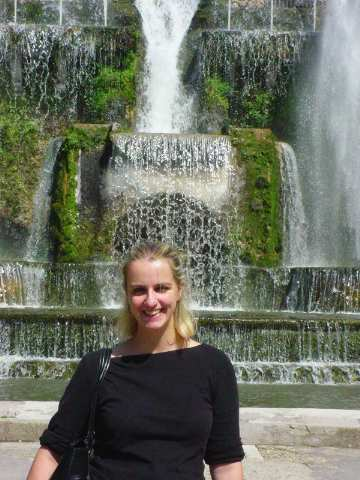
\includegraphics[width=0.45\columnwidth]{../figures/researchmicros-000.jpg}
  \hfill
  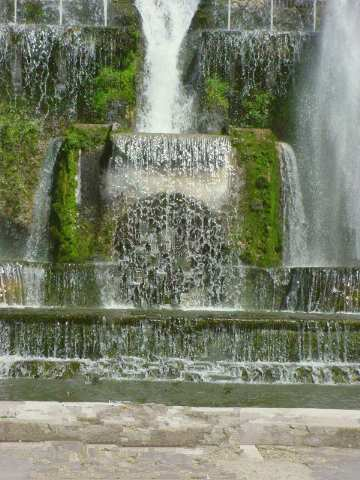
\includegraphics[width=0.45\columnwidth]{../figures/researchmicros-001.jpg}
\caption{Removing large objects from images (image obtained from \cite{Criminisi2004})}
\end{figure}

Traditionally, inpainting is a process undertaken by professional conservator-restorators.

\subsection{Subsubsection 1} % Sub-sub-section


\begin{figure}[H] % Example image
\center{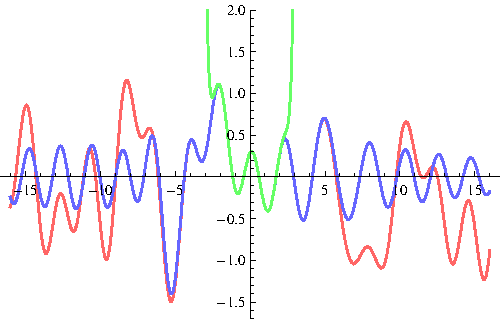
\includegraphics[width=0.5\linewidth]{approx}}
\caption{Example image.}
\label{fig:speciation}
\end{figure}

%------------------------------------------------

\subsubsection{Subsubsection 2} % Sub-sub-section


\subsection{Literature review}

%----------------------------------------------------------------------------------------
%	MAJOR SECTION 1
%----------------------------------------------------------------------------------------

\section{Research Proposal} % Major section


%------------------------------------------------

\subsection{Methodology} % Sub-section

\subsubsection{Evaluation framework} % Sub-sub-section

%------------------------------------------------

\subsubsection{Subsubsection 3} % Sub-sub-section

\subsection{Plan}

\subsection{Timetable}

\begin{description} % Numbered list example

\item[First] \hfill \\

\item[Second] \hfill \\

\item[Third] \hfill \\

\end{description} 


%----------------------------------------------------------------------------------------
%	BIBLIOGRAPHY
%----------------------------------------------------------------------------------------

\bibliography{../bibliography}

%----------------------------------------------------------------------------------------
%	APPENDIX
%----------------------------------------------------------------------------------------

\appendix

\section{Code}

%----------------------------------------------------------------------------------------
%	INDEX
%----------------------------------------------------------------------------------------

\printindex

%----------------------------------------------------------------------------------------

\end{document}